\documentclass{beamer}
\usepackage{default}
\usetheme{Boadilla}
\useoutertheme{infolines}
\usecolortheme{tum}
\usepackage{helvet}
\usepackage{pdfpcnotes}
\usepackage{amsmath}
\usepackage{amsthm}
\usepackage{amsfonts}
\usepackage{cancel}


\usepackage{graphicx}
\usepackage[utf8]{inputenc}
\usepackage[english]{babel}

\definecolor{mygreen}{RGB}{116,167,85}
\definecolor{myred}{RGB}{188,46,52}
\definecolor{myblue}{RGB}{65,81,140}



\usepackage[backend=bibtex, style=authoryear]{biblatex}
\addbibresource{literature.bib}


\usepackage{setspace}
\usepackage{multirow}
\usepackage{color}
\usepackage{xcolor}
\usepackage{textcomp}
\usepackage{listings}
\usepackage{siunitx}
\usepackage{subfigure}
\usepackage{tikz}
\usepackage{tikzscale}


\usepackage{fixme} 

\let\oldfootnote\footnote
\renewcommand\footnote[1][]{\oldfootnote[frame,#1]}

%commands
\newcommand\blfootnote[1]{%
	\begingroup
	\renewcommand\thefootnote{}{\footnote{{#1}}}%
	\addtocounter{footnote}{-1}%
	\endgroup
}

\let\pnote\pnote

\usetikzlibrary{shapes.multipart}
\tikzstyle{state}=[shape=circle,draw=blue!50,fill=blue!20]
\tikzstyle{observation}=[shape=rectangle,draw=orange!50,fill=orange!20]
\tikzstyle{lightedge}=[<-,dotted]
\tikzstyle{mainstate}=[state,thick]
\tikzstyle{mainedge}=[<-,thick]

%opening

\title[disorder prediction]{Prediction of Disordered Protein Regions}
\subtitle{}
\date{2016-06-16}
\author{Nicola Palandt, Gregor Sturm}
\institute[rostlab]{Rostlab, Technical University of Munich}


\begin{document}

\maketitle

\begin{frame}{We extracted fragments from Disprot.}
\begin{center}
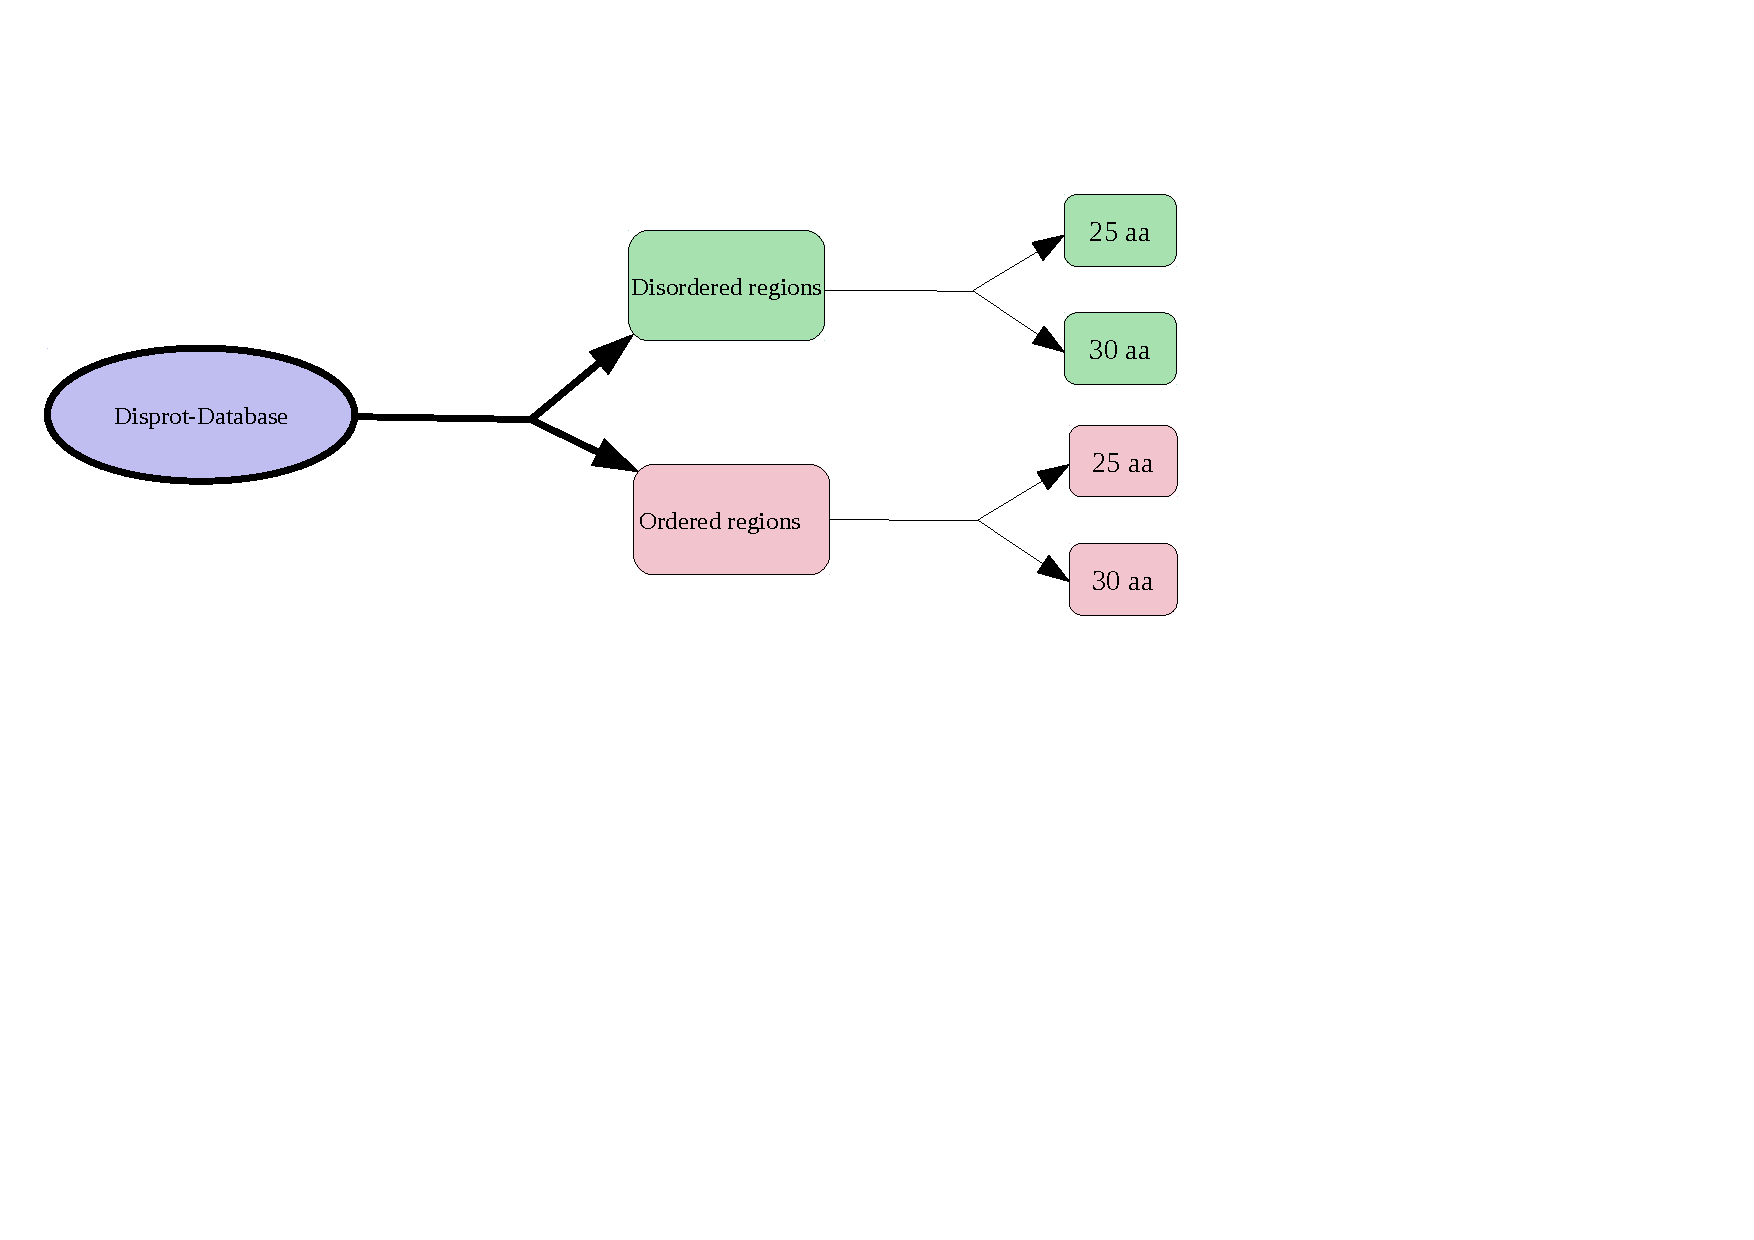
\includegraphics[width=.7\textwidth]{img/schema_preprocessing.pdf}\newline
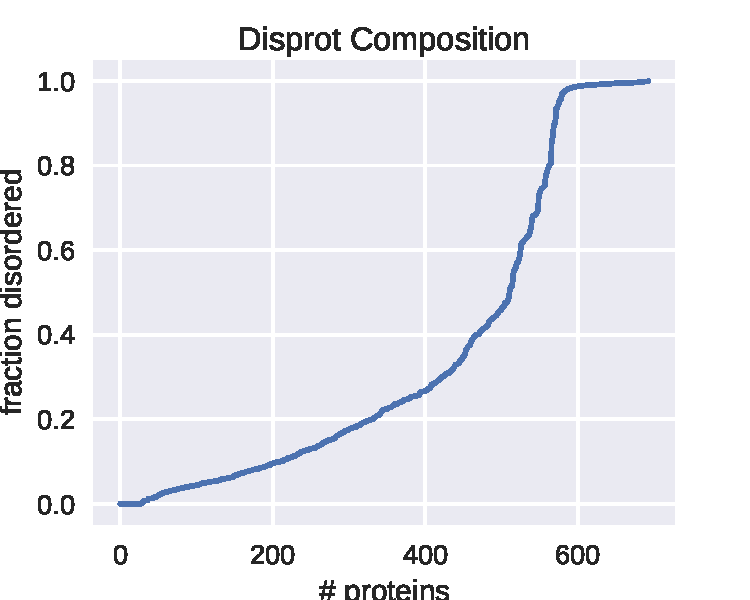
\includegraphics[width=.4\textwidth]{img/disprot_comp.pdf}
\end{center}
\end{frame}

\begin{frame}{We performed a parameter optimization on the profile kernel.}
Optimal combination: $L=1, Y=3$:
\begin{columns}[t]
\column{.5\textwidth}{
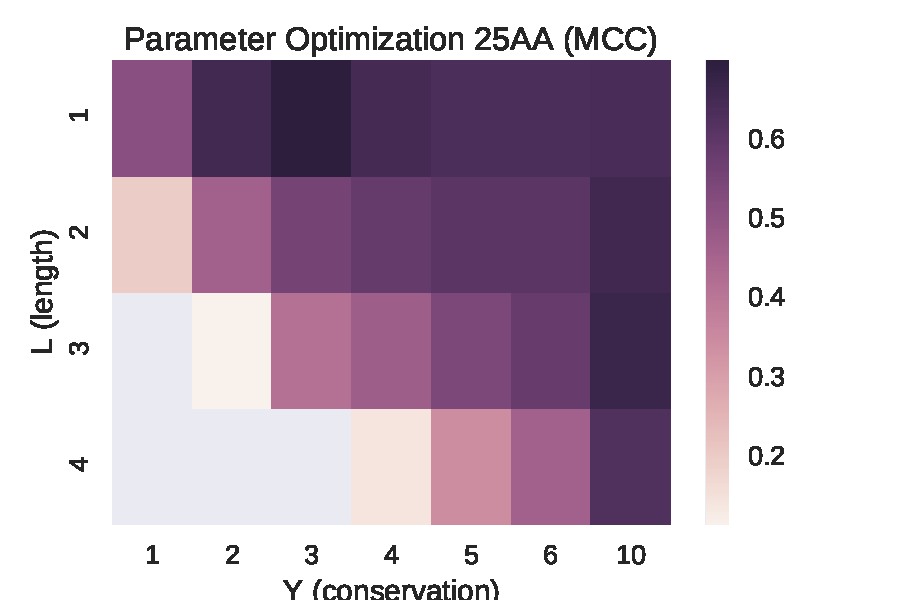
\includegraphics[width=\linewidth]{img/mcc25.pdf}}
\column{.5\textwidth}{
\pause
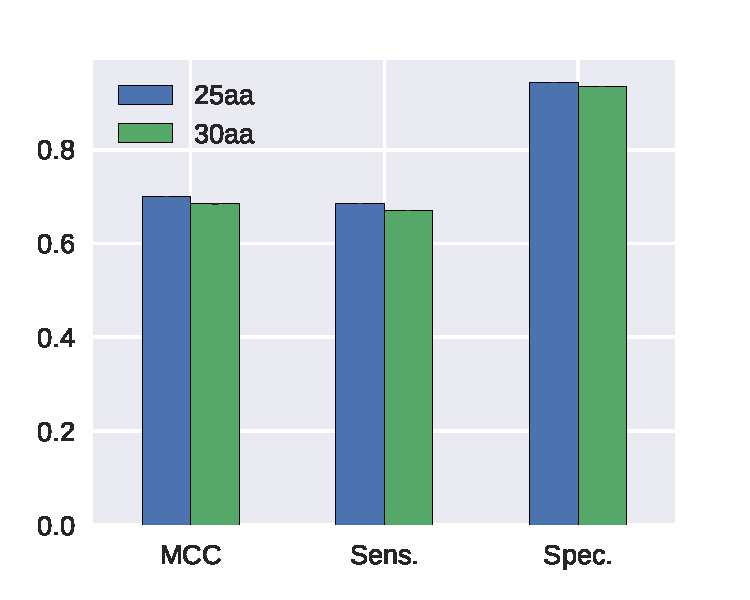
\includegraphics[width=\linewidth]{img/perfs_best.pdf}
}
\end{columns}
\end{frame}

\begin{frame}{We tested our method against other approaches.}
\begin{columns}[t]
\column{.5\textwidth}{
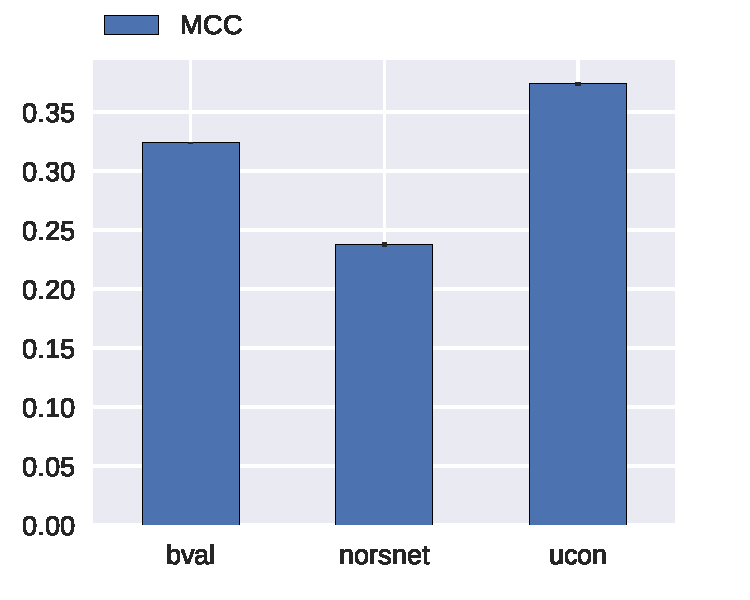
\includegraphics[width=\linewidth]{img/mcc_testset.pdf}}
\column{.5\textwidth}{
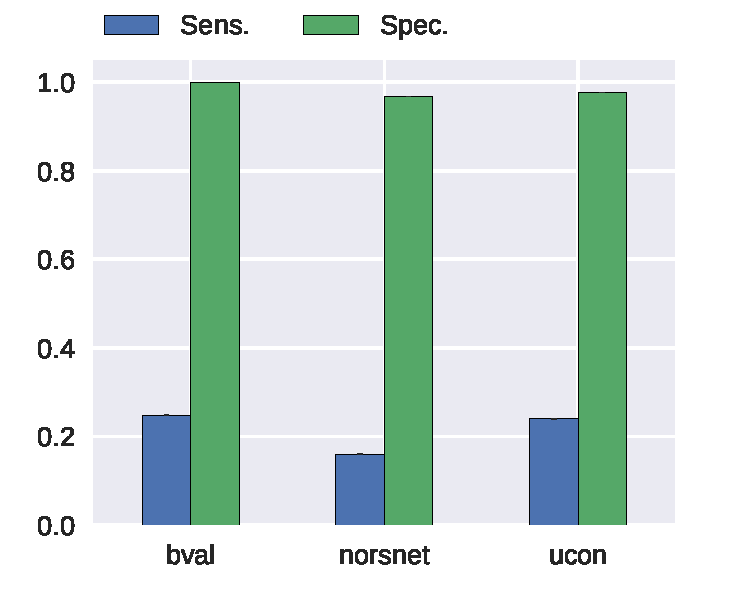
\includegraphics[width=\linewidth]{img/sens_spec_testset.pdf}
}
\end{columns}
\end{frame}

\begin{frame}{Is the amino acid composition driving disorder?}
\begin{center}
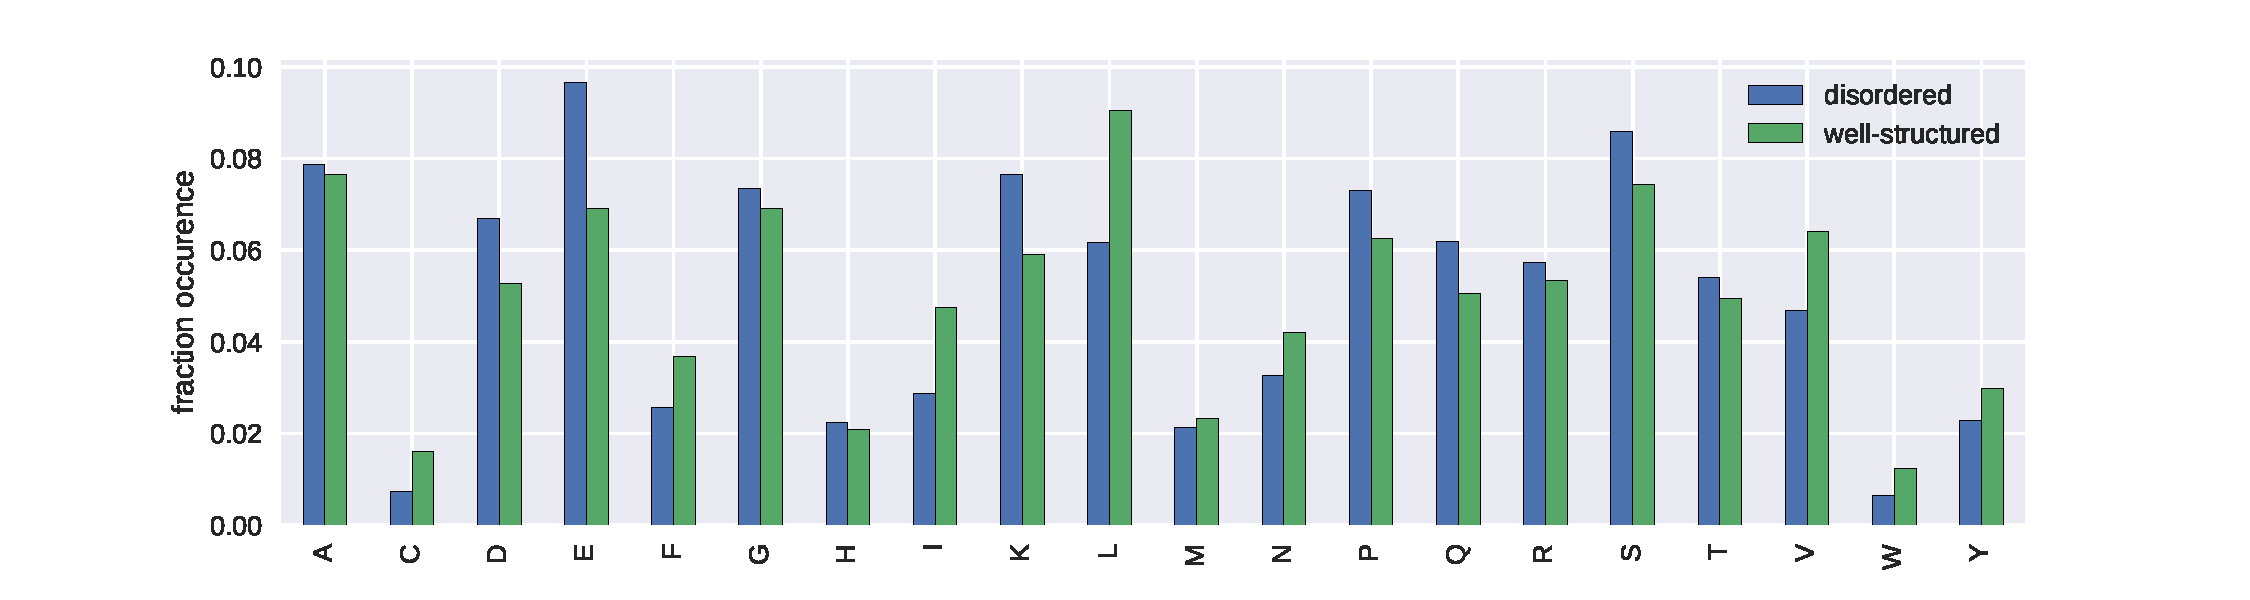
\includegraphics[width=\textwidth]{img/aacomp.pdf}\newline
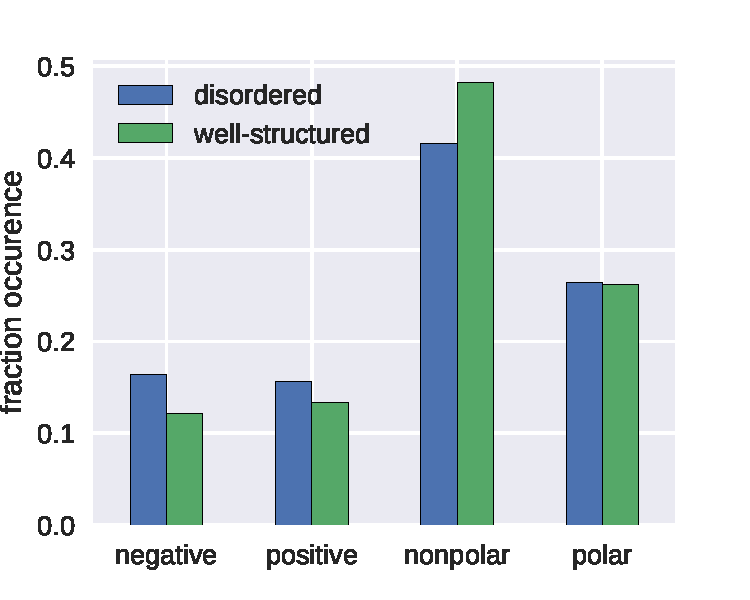
\includegraphics[width=.4\textwidth]{img/aacomp_group.pdf}
\end{center}
\end{frame}



%\begin{frame}[allowframebreaks]
%\frametitle{References}
%\printbibliography
%\end{frame}

\end{document}
